\documentclass[../../main/main.tex]{subfiles}

\begin{document}

\section{Theory}
\label{sec:theory}



\subsection{Neural network}
\label{sec:neural-network}


A neural network consists of neurons, also called nodes, in a network which are inspired by the neurons in the brain \cite{morten}. The node takes input from the neighbouring  nodes and uses an activation function \(f\) to calculate the input nodes with the weights \(w\) that describes the connection between the nodes. The output \(y\) that is connected to a set of nodes \(x_i\) with weights \(w_i\) is gives an
\begin{equation}
  \label{eq:art-neurons}
  y = f\left( \sum_{i=1}^n w_ix_i\right) = f(u)
\end{equation}
and is illustrated in Figure \ref{fig:neuron}a. A neural network consist of layers with connected neurons, or also called nodes.
\begin{figure}[H]
  \centering
  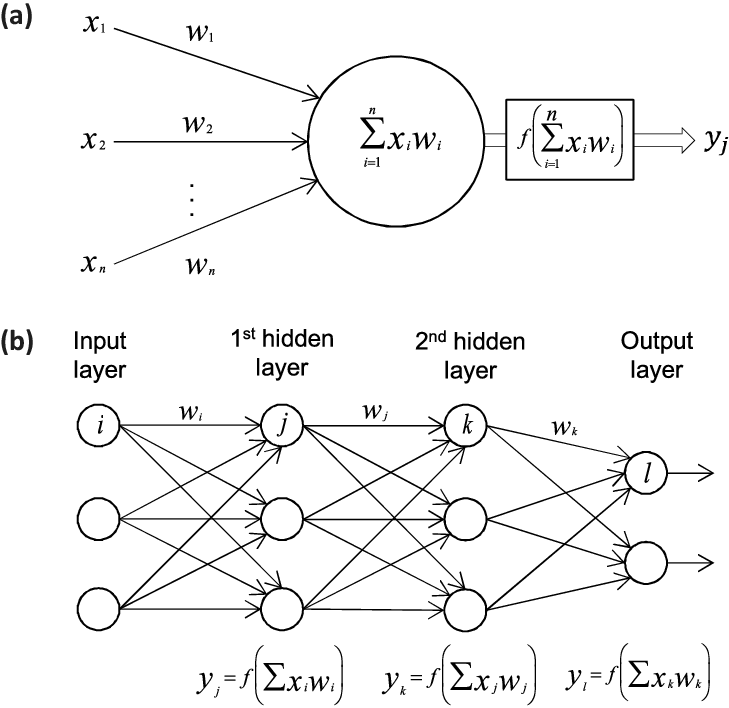
\includegraphics[width=\linewidth]{../../figures/neuron.png}
  \caption{Neural network, from \cite{morten}}
  \label{fig:neuron}  
\end{figure}

The output \(y\) of a node is given via the activation function \(f\) as
\begin{equation}
  \label{eq:2}
  y = f\left( \sum_{i=1}^n w_ix_i + b_i\right) = f(z),
\end{equation}
where \(x_i\) is the input from the neurons in the preciding layers, and \(b_i\) is called the \emph{bias} which is included in the case of a zero weight \(w_i\) or input \(x_i\) in the activation function. In e.g the first layer of a neural network we calculate the weighted sum \(z_i^1\) for each node in the layer over the input coordinates \(x_j\) as
\begin{equation}
  \label{eq:weighted-sum}
  z^1_i=\sum_{j=1}^M w_{ij}^1x_j+b_i^1,
\end{equation}
where \(M\) denotes all the possible inputs to a given node \(i\) in the first layer. We call the layer \emph{fully connected} if all the nodes in the layer takes all the nodes from the previous layer as input, and \(M\) is then equal to the number of nodes in the previous layer. The activation function \(f_i\) for each node \(i\) takes the value of the activation function in Eq. \eqref{eq:weighted-sum} and gives us the output \(y_i^1\) of all neurons in layer 1 as
\begin{equation}
  \label{eq:6}
  y_i^1 = f(z^1_i) = f \left( \sum_{j=1}^M w_{ij}^1x_j+b_i^1 \right), 
\end{equation}
with the assumption that all the nodes in the same layer has the same activation function, and we therefore drop the subsctipt \(i\) on \(f_i\). If the layers has different activation functions we can denote it with a superscript \(l\) for a layer \(l\). The output of the node \(i\) for layer \(l\) therefore becomes
\begin{equation}
  \label{eq:layer-output}
  y_i^l = f(z^l_i) = f \left( \sum_{j=1}^{N_{l-1}} w_{ij}^ly_j^{l-1}+b_i^l \right), 
\end{equation}
where \(N_{l-1}\) is the number of nodes in the previous layer if the layer is fully connected. With Eq. \eqref{eq:layer-output} we can calculate the output \(y_i^l\) from layer \(l\) from the output \(y_i^{l-1}\) from the previous layer \(l-1\). Given the input \(x_n\) from the input layer with \(n\) nodes, the output from layer \(l+1\) can therefore be calculated as
\begin{align}
  \label{eq:layer-output-l}
  y_i^{l+1} = f^{l+1}\Biggl[&\sum_{j=i}^{N_l} w_{ij}^{l+1}f^l\Biggl(\sum_{j=i}^{N_{l-1}} w_{jk} \Biggl(
  \notag \\
                            ...&f^1\Biggl(\sum_{j=i}^{N_0} w_{mn}^1x_n + b_m^1\Biggr) ... \Biggr) + b_j^l\Biggr) + b_i^{l+1}\Biggr].
\end{align}
Eq. \eqref{eq:layer-output-l} shows that the MPL is nothing more than an analytic function which is given by the real valued map \(\hat{x}\in\mathbb{R}^n \rightarrow\hat{y}\in\mathbb{R}^m\). This concludes the feed forward method. Now we go over to the famous back propagation algorithm (cite) which is used to update the weights and biases in the neural network. To summarize the weights \(w_{ij}^l\) and biases \(b_j\) are updated according to
\begin{align}
  w_{jk}^l &\leftarrow w_{jk}^l - \eta\delta_j^ly_k^{l-1} \label{eq:uptate-weight} \\
  b_j^l &\leftarrow b_j - \eta\delta_j^l \label{eq:uptate-bias},
\end{align} 
where \(\delta_j^l\) is the error that is calculated from the derivative of the cost function \(\mathcal{C}\) and \(\eta\) is the learning rate. A more detailed description of the back propagation algorithm can be found in \cite{morten}.
\subsection{Discovery statistics and the profile likelihood ratio in particle physics}
\label{sec:statistics} 

In particle physics we often test a so called \emph{background hypythis} that test the physics we know against the \emph{signal + background hypotisis} that test unknown physics that could possible discover by rejecting the background hypothisis. One way of doing this is to calculate the discover significance \(Z\) which counts the number of standard derivations and is the square of some test statistics \(q_0\). In a search region where there are \(b\) background events and \(s\) signal events the discover significance is given as
\begin{equation}
  \label{eq:discover-sig}
  Z = \sqrt{2(s+b)\ln\left(1 + \frac{s}{b}\right) - s},
\end{equation}
and is often used in particle physics. Another way of using the test statistics is to use the \emph{profile likelihood ratio} and the signal strength \(\mu\) which measures how strong the signal is.
To test a hypothisis value for the signal strength \(\mu\) we use the \emph{profile likelihood ratio} \cite{Cowan_2011}
\begin{equation}
  \label{eq:profile-likelihood-ratio}
  \lambda(\mu) = \frac{L(\mu,\hat{\hat{\bm{\theta}}})}{L(\hat{\mu},\bm{\hat{\theta}})},
\end{equation}
where in the numerator the value of \(\theta\) that maximizes \(L\) for a specific \(\mu\) is denoted by the quantity \(\hat{\hat{\bm{\theta}}}\), and is therefore the conditional maximum-likelihood (ML) estimator that estimates \(\bm{\theta}\), and therefore a function of \(\mu\). The denominator is the unconditional likelihood function where \(\hat{\mu}\) and \(\bm{\hat{\theta}}\) are their ML estimators.

By Wilks' theorem we can use the test statistics 

\begin{equation}
  \label{eq:wilks-test}
  q_0=\begin{cases}
             -2\ln \lambda(0), & \text{if \(n > b\),}\\
             0, & \text{otherwise}
           \end{cases}
\end{equation}

The appropiate likelihood ratio in searches for new particles is the ratio of the likelihood for the signal+background hypothisis and the likelihood for the background hypothisis and is given generally as
\begin{equation}
  \label{eq:discovery-likelihood-ratio}
  Q = \frac{L_{s+b}(\mu)}{L_b}
\end{equation}

This likelihood ratio can be expressed in terms of the background only likelihood function \(L_b\) and signal only density function \(L_s\) and is given as \cite{Read:2000ru}
\begin{equation}
  \label{eq:discovery-likelihood-ratio-s-b}
  Q = e^{-s_{exp}}\prod_{i=1}^n\left(1+\frac{s_{exp}L_s(x_i)}{b_{exp}L_b(x_i)}\right),
\end{equation}
where \(b_{exp}\) and \(s_{exp}\) are the expected background and signal events, and the product is taken over a given experimental result \(x_i\) for each event \(i\) over the total number of events \(n\). We insert the signal strength parameter \(\mu\) in front of the expected number of signal events \(s_{exp}\), which gives us
\begin{equation}
  \label{eq:discovery-likelihood-ratio-mu}
  Q(\mu) = e^{-\mu s_{exp}}\prod_{i=1}^n\left(1+\frac{\mu s_{exp}L_s(x_i)}{b_{exp}L_b(x_i)}\right).
\end{equation}
The profile log-likelihood ratio \(t(\mu)\) is therefore equal to
\begin{align}
  \label{eq:discovery-likelihood-ratio-mu}
  t(\mu) &= -2\ln Q(\mu) \notag \\
  &= \mu s_{exp} - \sum_{i=1}^n\left(1+ \frac{\mu s_{exp}L_s(x_i)}{b_{exp}L_b(x_i)}\right),
\end{align}
when expressed in terms of \(L_s\) and \(L_b\). In the profile likelihood ratio in Eq. (\ref{eq:profile-likelihood-ratio}) we see that the estimator value that maximizes the signal+background likelihood function is \(\hat{\mu}=1\) in the unconditional likelihood function in the denominator in Eq. (\ref{eq:profile-likelihood-ratio}). Using this the derivation in Eq. .. in Appendix gives us the relation
\begin{align}
  -2\ln \lambda(\mu) &= -2\ln Q(\mu) + 2\ln Q(1) \notag \\
             &= t(\mu) - t(1),   \label{eq:relation-likelihood}
\end{align}
If the estimated value \(\hat{\mu}\) that maximises an \emph{approximated} signal+background likelihood function is not equal to the expexted estimate \(\hat{\mu} = 1\), as used to derive Eq. (\ref{eq:relation-likelihood}), we use the estimated value \(\hat{\mu}\) instead in the relation above. This gives us the same relation as above, but where we replace 1 by \(\hat{\mu}\) in the last term
\begin{align}
  -2\ln \lambda(\mu) &= -2\ln Q(\mu) + 2\ln Q(\hat{\mu}) \notag \\
             &= t(\mu) - t(\hat{\mu}),   \label{eq:relation-likelihood-approx}
\end{align}
which is the more general form. This gives us the test statistic
\begin{equation}
  \label{eq:5}
  q_0=\begin{cases}
        t(0) - t(\hat{\mu}), & \text{if \(n > b_{exp}\),}\\
        0, & \text{otherwise},
      \end{cases}
\end{equation}
and the discovery significance \(Z\) is then given as
\begin{equation}
  \label{eq:discovery-sig-likelihood}
  Z = \sqrt{q_0} = \begin{cases}
        \sqrt{t(0) - t(\hat{\mu})}, & \text{if \(n > b_{exp}\),}\\
        0, & \text{otherwise}.
      \end{cases}
\end{equation}

\subsection{Likelihood estimation}
\label{sec:likel-estim}

The likelihood ratio function can be estimated by a neural network with a method developed by G. V. Moustakides and K. Basioti \cite{moustakides2019training} which transforms the output of the neural network to a likelihood ratio by solving an optimalization problem. For a random vector \(X\) with the probability function \(f_0(X)\) we want to optrimalisze the following loss function
\begin{equation}
  \label{eq:likilhood-loss}
  \mathcal{J}(u) = \mathrm{E_0}[\phi(u(X)) + \mathrm{r}(X)\psi(\mathrm{u}(X))],
\end{equation}

where \(\mathrm{E_0[\cdot]}\) is the expectation value w.r.t. \(f_0(X)\), and \(\phi(z)\) and \(\psi(z)\) are scalar functions of the scalar \(z\), and \(\mathrm{u}(X)\) and \(\mathrm{r}(X)\) are scalar functions of \(X\) were \(\mathrm{r}(X)\) takes values in a \emph{known} interval \(\mathcal{I}_r\). The optimalization problem we want to solve is
\begin{equation}
  \label{eq:min-likelihood-loss}
  \min_{\mathrm{u}(X)} \mathcal{J}(u) = \min_{\mathrm{u}(X)} \mathrm{E_0}[\phi(u(X)) + \mathrm{r}(X)\psi(\mathrm{u}(X))],
\end{equation}
such that when we have a known scalar function \(\omega(r)\) of the scalar \(r\), we want to determine the two functions \(\phi(z)\) and \(\theta(z)\) such that the global minimizer in Eq. (\ref{eq:min-loss}) is equal to
\begin{equation}
  \label{eq:min-likelihood-conditon}
  \mathrm{u}(X) = \omega(\mathrm{r}(X)).
\end{equation}
In \cite{moustakides2019training} they show that the nessesary condition to achive the optimilization that satisfies this condition is that
\begin{equation}
  \label{eq:likelihood-condition-1}
  \phi^\prime(\omega(\mathrm{r}))+ \mathrm{r} \psi^\prime(\omega(\mathrm{r})) = 0.
\end{equation}
If \(\omega(r)\) is stighly monotone we also have the result
\begin{equation}
  \label{eq:likelihood-condition-stright}
  \phi^\prime(\omega(\mathrm{r}))+ \omega^{-1}(z) \psi^\prime(\omega(\mathrm{r})) = 0,
\end{equation}
for \(z\in\omega(\mathcal{I}_r)\) where \(\omega^{-1}(z)\) is the inverse of \(r\).
They further show that when we chose a function \(\rho(z)\) with the condition \(\rho(z) < 0\) for all \(z \in \omega(\mathcal{I}_r)\) and define \(\phi(z)\) and \(\theta(z)\) as
\begin{equation}
  \label{eq:likelihood-rhp}
  \psi^\prime(z) = \rho(z), \text{ and } \phi^\prime(z) = \omega^{-1}(z)\rho(z),
\end{equation}
then the minima of \(\phi(z) + r\theta(z)\) in Eq. (\ref{eq:min-likelihood-loss}) for \(z\in\omega(\mathcal{I}_r)\) is uniquely located at \(z = \omega(r)\). This is what we wanted to achive in Eq. (\ref{eq:min-likelihood-conditon}). When we chose
\begin{equation}
  \label{eq:4}
  \omega(z) = \frac{z}{z+1} \text{ and } \rho(z) = -\frac{1}{z}, 
\end{equation}
and use Eq. (\ref{eq:likelihood-rhp}) we get the following expressions for \(\phi(z)\) and \(\theta(z)\),
\begin{equation}
  \label{eq:1}
  \phi(z) = - \log{(1 - z)} \text{ and } \psi(z) = - \log{(z)}.
\end{equation}
This combination of \(\phi(z)\) and \(\theta(z)\) gives us the binary cross-entropy method and is among the most popular methods for classification problems.
When we define the scalar function \(\mathrm{r}(X)\) in Eq. (\ref{eq:likilhood-loss}) to be the likelihood ratio
\begin{equation}
  \label{eq:7}
  \mathrm{r}(X) = \frac{f_1(X)}{f_0(X)},
\end{equation}
of two probability distributions \(f_0(X)\) and \(f_1(X)\) the loss function \(\mathcal{J}(u)\) in Eq. (\ref{eq:likilhood-loss}) becomes
\begin{align}
  \label{eq:likelihood-loss-2}
  \mathcal{J}(u) &= \mathrm{E_0}[\phi(u(X)) + \mathrm{r}(X)\psi\big(\mathrm{u}(X)\big)] \notag \\
       &= \mathrm{E_0}[\phi(u(X))] + \mathrm{E_1}[\psi\big(\mathrm{u}(X)\big)],
\end{align}
where the expextation values \(\mathrm{E_0}\) and \(\mathrm{E_1}\) are w.r.t the probability functions \(f_0(X)\) and \(f_1(X)\) respectively. 
We are now interested in finding a way of using  a neural network to estimate the transformation \(\omega(\frac{f_1(X)}{f_0(X)})\) when we have two data samples \(\{X_1^0,...,X^0_{n_0}\}\) and \(\{X_1^1,...,X_{n_1}^1\}\) that are sampled from the \emph{unknown} probability densities \(f_0(X)\) and \(f_1(X)\) respectively, and when \(\omega(r)\) is a \emph{known} scalar function. Two approximations is needed to do this. For the first one we replace the statistical expectation values in Eq. (\ref{eq:likelihood-loss-2}) with the averages over the available data, while for the second we replace the function \(\mathrm{u}(X)\) with the output of a neural network \(\mathrm{u}(X,\theta)\), where \(\theta\) summatizes the network parameters. The first approximation requires a dataset with a large sample size, while the second approximation requires that the neural network is sufficently rich such that it can approximate any non-linear function. 
When applying the two approximations above, the loss function in Eq. (\ref{eq:likelihood-loss-2}) is approximated to
\begin{equation}
  \label{eq:1}
  \mathcal{J}(u) \approx \hat{\mathcal{J}}(\theta) = \frac{1}{n_0}\sum_{i=1}^{n_0} \phi(\mathrm{u}(X_i^0,\theta)) + \frac{1}{n_1}\sum_{i=1}^{n_1} \phi(\mathrm{u}(X_i^1,\theta))
\end{equation}
The optimalization problem is now transformed into an optimalization problem over the neural network parameters \(\theta\) as
\begin{align*}
  \min_{\mathrm{u}(X)} \mathcal{J}(u) &\approx \min_{\theta} \hat{\mathcal{J}}(\theta) \\
                            &= \min_{\theta}\left\{ \frac{1}{n_0}\sum_{i=1}^{n_0} \phi(\mathrm{u}(X_i^0,\theta)) + \frac{1}{n_1}\sum_{i=1}^{n_1} \phi(\mathrm{u}(X_i^1,\theta))\right\},
\end{align*}
and when optimized the optimal parameters \(\theta_o\) will give a neural network that has approximated the function \(\omega(r)\), that is
\begin{equation}
  \label{eq:9}
  \mathrm{u}(X,\theta_o) \approx \omega(\mathrm{r}(X)),
\end{equation}
provided that it does not reach a local minima.

\subsection{Estimating the profile log-likelihood ratio with neural network}
\label{sec:estim-prof-log}

We can use the method of estimating a likelihood ration described in the previous section when discovering new particles by estimating the profile log-likelihood ratio in Eq. (\ref{eq:profile-likelihood-ratio}). When we are interested to test the signal+background hypothisis against the background only hypothisis, which is given in the likelihood ratio function in Eq. (\ref{eq:discovery-likelihood-ratio-mu}), the likelihood ratio \(L_s/L_b\) is optimal to estimate when we have two datasets \(X_s\) and \(X_b\) which contains the signal and background data respectively
\end{document}
